\documentclass[14pt]{beamer}

\usepackage{listings}
\usepackage{tikz}
\usetikzlibrary{positioning}
\usetikzlibrary{arrows.meta}
\usepackage{pgfplots}

% presentation themeing
\setbeamertemplate{bibliography item}{\insertbiblabel}


% Julia listings definition
% Definition based on https://tex.stackexchange.com/a/212794/149437
% Original definition (c) 2014 Jubobs
\lstdefinelanguage{Julia}
  {morekeywords={abstract,break,case,catch,const,continue,do,else,elseif,
      end,export,false,for,function,immutable,import,importall,if,in,
      macro,module,otherwise,quote,return,switch,true,try,type,typealias,
      using,while,where},
   sensitive=true,
   alsoother={$},
   morecomment=[l]\#,
   morecomment=[n]{\#=}{=\#},
   morestring=[s]{"}{"},
   morestring=[m]{'}{'},
}[keywords,comments,strings]


\title[JuliaPetra]{Obtaining Performance from a Julia-Implementation of Trilinos Data Libraries}
\author{Neil Lindquist}
\date[SIAM CSE19]{SIAM Conference on Computational Science and Engineering\\February 27th 2019}


\begin{document}
\frame{\titlepage}
\begin{frame}
	\frametitle{Julia}
	\nocite{Bezanson:2017:FreshApproach}
	\begin{itemize}
		\item High Level
		\item Compiles to efficient machine code
	\end{itemize}
	%TODO consider if Wilkins prize should be mentioned
	%TODO should LLVM be mentioned?
	\note{
		\item high level language
		\item can perform on par with C
		\begin{itemize}
			\item type inferencing
			\item compiling each concrete method signature
		\end{itemize}
	}
\end{frame}
\begin{frame}
	\frametitle{Petra Object Model}
	\nocite{Heroux:2005:Trilinos}
	\begin{itemize}
		\item Family of sparse linear algebra frameworks
		\item Underlying data libraries for Trilinos
		\item 3 existing implementations
	\end{itemize}
	\note{
		\item The Petra libraries are the underlying data structures used by Trilinos
		\item 3 implementations
		\begin{itemize}
			\item Epetra - original, portable version
			\item Tpetra - newer, uses more advanced C++ features
			\item Jpetra - experiemental, pure java version
		\end{itemize}
	}
\end{frame}
\begin{frame}
	\frametitle{JuliaPetra Organization}
	\nocite{Github:MPI}
	\centering
	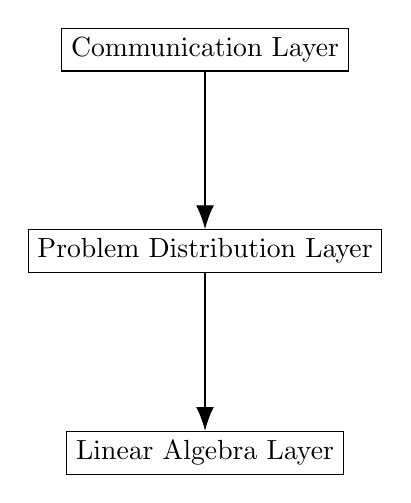
\begin{tikzpicture}
		\node[rectangle, draw=black] (CommLayer) {Communication Layer};
		\node[rectangle, draw=black] (DistLayer) [below=2cm of CommLayer] {Problem Distribution Layer};
		\node[rectangle, draw=black] (LALayer) [below=2cm of DistLayer] {Linear Algebra Layer};
		\draw[-{Latex[length=3mm]}] (CommLayer.south) -- (DistLayer);
		\draw[-{Latex[length=3mm]}] (DistLayer.south) -- (LALayer);
	\end{tikzpicture}
	\note{
	\item Communication layer handles the movement of data between processes
	\begin{itemize}
		\item Can be implemented with any Single-Program-Multiple-Data parallel system
		\item There are serial and MPI implementations
		\item MPI.jl is used for MPI communication
	\end{itemize}
	\item Distribution layer managed how the parts of the problem are distributed
	\item Linear Algebra layer provides the iterfaces for vector and linear transformation objects
	}
\end{frame}
\begin{frame}[fragile]
	\frametitle{JuliaPetra Example of the Power Method}
	\begin{lstlisting}[
		language         = Julia,
		basicstyle       = \ttfamily\footnotesize,
		keywordstyle     = \bfseries\color{blue},
		stringstyle      = \color{magenta},
		commentstyle     = \color{ForestGreen},
		showstringspaces = false,
		mathescape]
function powerMethod(A::RowMatrix{Data}, $\epsilon$::Data)
        where {Data}
    q = DenseMultiVector{Data}(getRowMap(A), 1)
    z = DenseMultiVector{Data}(getRowMap(A), 1)
    randn!(z.data)
    r = DenseMultiVector{Data}(getRowMap(A), 1)
    while true
        normz = norm2(z)[1]
        @. q = z/normz
        apply!(z, A, q)
        $\lambda$ = dot(q, z)[1]
        @. r = z - $\lambda$*q
        if norm2(r)[1] < $\epsilon$
            return $\lambda$
        end
    end
end
	\end{lstlisting}
\end{frame}
\begin{frame}
	\frametitle{Performance Comparison}
	\nocite{Github:DA,Gu:2000:PowerMethod}
	\centering
	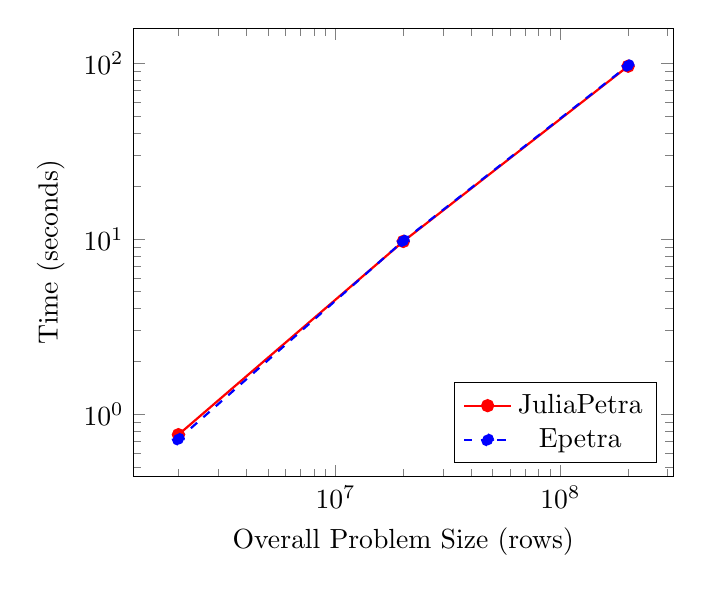
\begin{tikzpicture}
		\begin{loglogaxis}[
			xlabel = {Overall Problem Size (rows)},
			ylabel = {Time (seconds)},
			legend pos = south east
			]
			\addplot[color=red,mark=*,thick] coordinates{(2000000,0.76502)(20000000,9.67784)(200000000,96.6538)};
			\addlegendentry{JuliaPetra}
			\addplot[color=blue,mark=*,thick,dashed]  coordinates{(2000000,0.72094)(20000000,9.74738)(200000000,97.4296)};
			\addlegendentry{Epetra}
		\end{loglogaxis}
	\end{tikzpicture}
	
	Performance of the power method for eigenvalues.
	\note{Results are for a tridiagonal matrix using a 20 core machine}
	\note{DistributedArrays.jl was significantly slower}
\end{frame}
\begin{frame}
	\frametitle{Optimizing JuliaPetra}
	%TODO Overview of optimizing Julia
\end{frame}
\begin{frame}
	\frametitle{Type Stability}
	\framesubtitle{Optimizing JuliaPetra}
	%TODO type stability \& inlining
\end{frame}
\begin{frame}
	\frametitle{Reducing Garbage Collection}
	\framesubtitle{Optimizing JuliaPetra}
	%TODO garbage collection reduction
	
	Is this really that important to the results?
\end{frame}
\begin{frame}
	\frametitle{Bounds Checks}
	\framesubtitle{Optimizing JuliaPetra}
	%TODO bounds checks
\end{frame}
\begin{frame}
	\frametitle{Conclusion}
	\begin{itemize}
		\item Julia is a promising fast, high level language
		\item JuliaPetra matches Epetra's performance
	\end{itemize}
	%TODO add conclusion note about optimization
\end{frame}
\begin{frame}[allowframebreaks]
	\frametitle{References}

\bibliographystyle{plain}
\bibliography{bibliography}

\end{frame}
\end{document}
